\documentclass[11pt]{beamer}
\usetheme{Warsaw} %tema beamer
\usecolortheme{default}
\usepackage[spanish]{babel}
\usepackage{multicol}
\usepackage{ragged2e} %para justificar el texto
\usepackage{graphics,graphicx,url,hyperref,doi}
\usepackage{adjustbox}
\usepackage[numbers, sort, compress]{natbib}

\setbeamertemplate{caption}[numbered]% agregar númeración a tablas y figuras
%\renewcommand{\figurename}{Figura} %para poner etiqueta Figura
%\renewcommand{\tablename}{Tabla} %para poner etiqueta Tabla
\begin{document}

\title[Defensa de Tesis  \hspace{35mm} \insertframenumber/\inserttotalframenumber]{Modelado y visualización de relaciones entre contaminantes del aire y salud pública}
\centering \institute[Institución]{\\Universidad Autónoma de Nuevo León \\Facultad de Ingeniería Mecánica y Eléctrica}
\author{Selene Berenice Prado Prado \\ Ing. en Tecnología de Software}
\begin{frame}
\begin{center}
\end{center}
\vspace{-1cm}
\titlepage
\end{frame}

\begin{frame}{Índice}
\transdissolve
\begin{center}
\begin{multicols}{2}
  \footnotesize{\tableofcontents}	
\end{multicols}
\end{center}
\end{frame}


\section{Introducción}

\begin{frame}{Introducción}
\begin{figure}[!h]
    \centering
	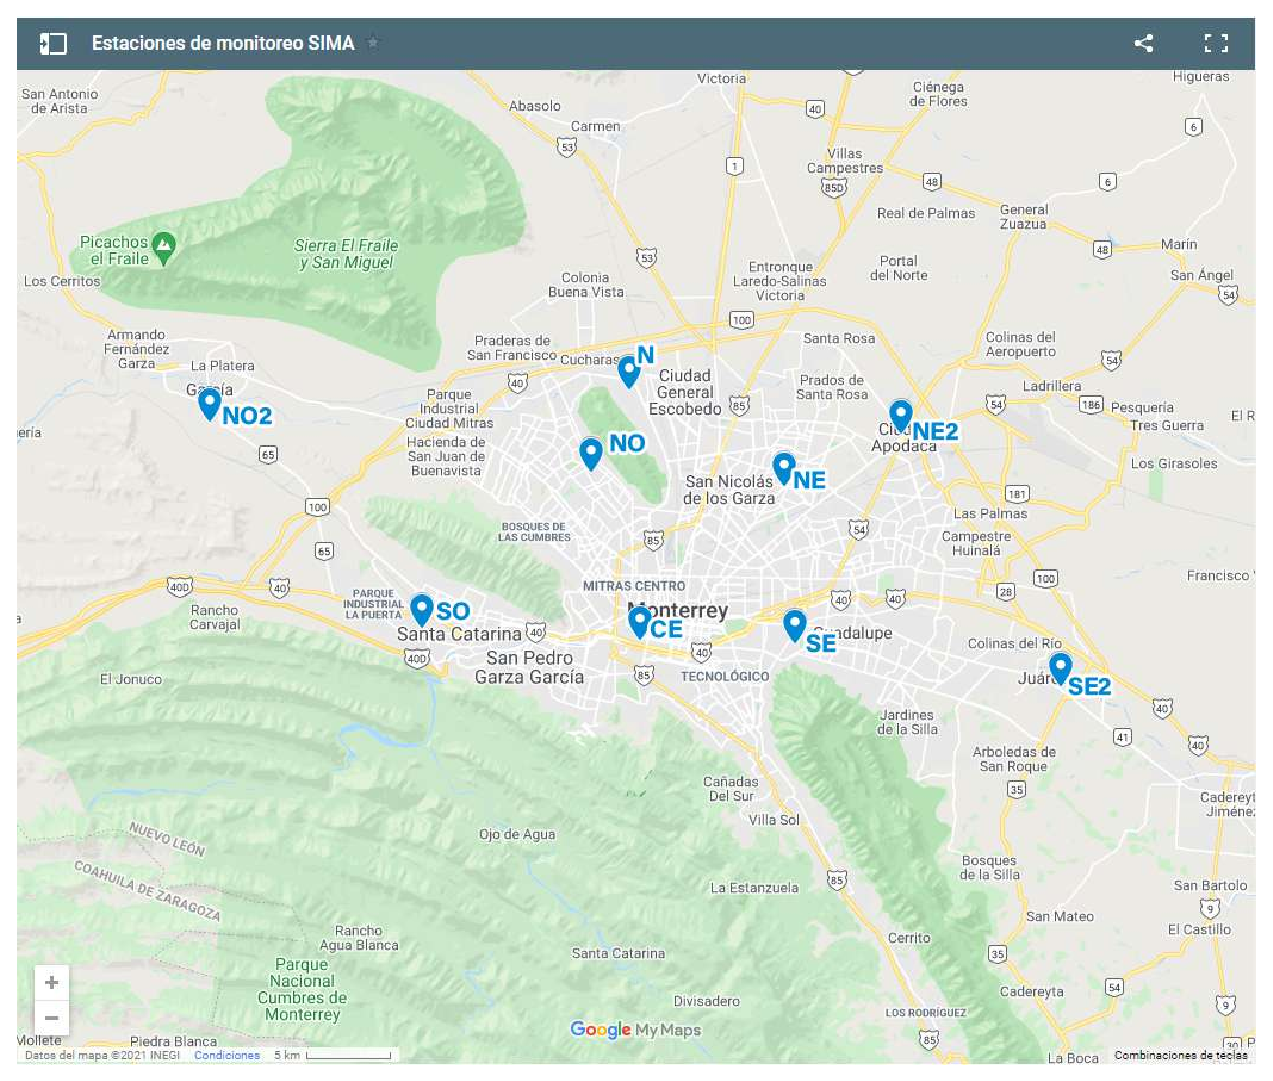
\includegraphics[trim=50 50 50 50,clip,width=0.55\textwidth]{mapa_estaciones}
	\label{fig:estaciones}
	\caption{Estaciones de monitoreo de la calidad del aire pertenecientes al Sistema Integral de Monitoreo Ambiental (SIMA) \cite{f2}.}
	\end{figure}
\end{frame}
%\subsection{Motivación}
%\begin{frame}{Motivación}
%\begin{block}{Motivación} \justifying
%Con el presente trabajo se busca aportar a la creación de nuevas herramientas que permitan observar y estudiar dichas relaciones con el fin de ayudar a tomar medidas adecuadas que permitan aminorar los efectos negativos de los contaminantes del aire en la salud.
%Aplicar técnicas avanzadas de \textbf{inteligencia artificial} y la \textbf{visión computacional} en \textbf{problemas forestales}.
%\end{block}
%\end{frame}
\subsection{Hipótesis}
\begin{frame}{Hipótesis}
\begin{block}{Hipótesis} \justifying
Los modelos de regresión permiten obtener gráficos donde se pueden observar las relaciones entre el número de ingresos hospitalarios y los niveles de contaminantes del aire.
%El procesamiento de imágenes automatiza procesos y reduce tiempos.
\end{block}
\end{frame}
\subsection{Objetivos}
\begin{frame}{Objetivos} 
\begin{block}{Objetivo general} \justifying
Generar, implementar y evaluar modelos que muestran las relaciones existentes entre contaminantes del aire y salud pública tiene la finalidad de apoyar a la implementación de estrategias que aminoran los efectos negativos de los contaminantes del aire en la salud de las personas. Con los modelos generados se puede tener una herramienta que permite identificar gráficamente las relaciones con solo proporcionarle el conjunto de datos.
%Generar un inventario forestal mediante el procesamiento de imágenes.
\end{block}
%\begin{block}{Objetivo específico} \justifying
%Automatizar procesos de las técnicas tradicionales para realizar \textbf{inventarios forestales}.
%\end{block}
\end{frame}


\section{Antecedentes}

\subsection{Monitoreo de calidad del aire}
\begin{frame}{Monitoreo de calidad del aire}
\begin{block}{Contaminantes del aire} \justifying
\begin{itemize}
	\item Monóxido de carbono (CO)
	\item Dióxido de azufre (SO$_2$)
	\item Óxidos de nitrógeno (NO$_x$)
	\item Ozono (O$_3$)
	\item Partículas de tamaño menor a 10 micrómetros (PM10)
	\item Partículas de tamaño menor a 2.5 micrómetros (PM2.5)
\end{itemize}
%En Nuevo León, México, las operaciones de la Red Automática de Monitoreo Atmosférico iniciaron en 1993. Dicha red en sus inicios contaba con cinco estaciones fijas de monitoreo continuo de monóxido de carbono (CO), dióxido de azufre (SO2), óxidos de nitrógeno (NOx), ozono (O3) y partículas de tamaño menor a 10 micrómetros (PM10).
\end{block}
\end{frame}
\subsection{Series de tiempo}
\begin{frame}{Series de tiempo}
\begin{block}{Definición de serie de tiempo} \justifying
Las series de tiempo se pueden definir como un conjunto de observaciones tomadas en un tiempo $t$ determinado. Los estudios de series de tiempo relacionan estadísticamente los cambios temporales en la repercusión de cambios en la concentración de un contaminante en la población \citep{r8}.
\end{block}
\end{frame}
\begin{frame}{Series de tiempo}
\begin{block}{Definición de semana epidemiológica} \justifying
Una semana epidemiológica es un estándar de medición temporal que se utiliza para comparar datos en ventanas de tiempo definidas. La primera semana epidemiológica del año termina el primer sábado de enero de cada año \citep{r7}.
\end{block}
\end{frame}
\subsection{Clasificación de enfermedades}
\begin{frame}{Clasificación de enfermedades}
\begin{block}{Clasificación Internacional de Enfermedades (CIE)} \justifying
Existe un instrumento estadístico y sanitario para identificar enfermedades llamado Clasificación Internacional de Enfermedades (CIE) que agrupa enfermedades en epidémicas, generales, locales ordenadas por origen geográfico, trastornos del desarrollo y lesiones \citep{r9}.
\end{block}
\end{frame}
\subsection{Regresión lineal}
\begin{frame}{Regresión lineal}
\begin{block}{Definición de regresión lineal} \justifying
La tendencia $w_0$ de una serie de tiempo puede ser obtenida a partir de una regresión lineal de la misma \citep{r10}. Una regresión lineal es una metodología inferencial supervisada que busca predecir valores $y$ dado un vector de variables de entrada $t$ por medio del ajuste de coeficientes $w$ de la función lineal: 
\begin{equation}
    \hat{y}(t,w) = w_0 + w_1x_1 + ... + w_tx_t.
    \label{eq1}
\end{equation}
\end{block}
\end{frame}
\subsection{Regresión lineal múltiple}
\begin{frame}{Regresión lineal múltiple}
\begin{block}{Definición de regresión lineal múltiple} \justifying
Un modelo de regresión múltiple es un modelo complemento de la regresión lineal simple, el cual tiene dos o más variables independientes $k$ que pueden influir en una variable dependiente $y$. \citet{r11} expresan la regresión múltiple mediante la siguiente ecuación:
\begin{equation}
    y = \beta_0 + \beta_1x_1 + ... + \beta_kx_k + \varepsilon.
    \label{eq2}
\end{equation}
\end{block}
\end{frame}


\section{Estado del arte}

\begin{frame}{Estado del arte}
\begin{table}[hbt!]
\centering
\caption[Comparación de trabajos]{Comparación de trabajos frente al desarrollado, donde $\checkmark$ indica que cumple con esta característica y  $\times$ no cumple con esta característica.}
\begin{adjustbox}{width=0.3\textwidth}
\begin{tabular}{|l|c|c|c|c|c|}
\hline
Trabajo & \rotatebox[origin=c]{90}{ Modelos de regresión lineal } & \rotatebox[origin=c]{90}{ Modelos de predicción } & \rotatebox[origin=c]{90}{ Evaluación de modelos } & \rotatebox[origin=c]{90}{ Estudio de contaminantes del aire } & \rotatebox[origin=c]{90}{ Estudio de problemas de salud }\\
	\hline
    \citet{r12} & \checkmark & $\times$ & $\times$ & \checkmark & \checkmark\\
    \hline
    \citet{r13} &  $\times$ & \checkmark & \checkmark & \checkmark & $\times$\\
    \hline
    \citet{r14} & \checkmark & \checkmark & $\times$ & \checkmark & \checkmark\\
    \hline
    \citet{r15} & \checkmark & \checkmark & $\times$ & \checkmark & \checkmark\\
	\hline    
    \citet{r16}& \checkmark & $\times$ & $\times$ & \checkmark & \checkmark\\
	\hline    
    \citet{r17} & $\times$ & \checkmark & \checkmark & \checkmark & \checkmark\\
	\hline    
    \citet{r18} & $\times$  & $\times$ & $\times$ & \checkmark & \checkmark\\
	\hline    
    \citet{r19} & \checkmark & \checkmark & $\times$ & \checkmark & \checkmark\\
	\hline    
    \citet{r20} &  \checkmark & \checkmark & $\times$ & \checkmark & \checkmark\\
	\hline    
    El presente trabajo & \checkmark & \checkmark & \checkmark & \checkmark & \checkmark\\
    \hline
\end{tabular}
\end{adjustbox}
\label{tab:Comparación de trabajos frente al desarrollado}
\end{table}
\end{frame}


\section{Solución propuesta}

\begin{frame}{Solución propuesta}
\begin{block}{Solución propuesta} \justifying
La solución propuesta se compone de cuatro fases principales: \textbf{recolección de datos, selección y agrupación de datos, visualización de la evolución de las variables e implementación de modelos}.
\end{block}
\end{frame}
\subsection{Herramientas}
\begin{frame}{Herramientas}
\begin{table}[H]
{\centering
	\caption{Herramientas utilizadas.}
	\begin{adjustbox}{width=0.9\textwidth}
	\begin{tabular}{|l|l|l|}
		\hline 
		Herramienta & Versión & URL\\
			\hline
			\texttt{Python} & 3.8.8 & \url{https://www.python.org/}\\
			\hline
			\texttt{Jupyter Notebook} & 6.3.0 & \url{https://jupyter.org/}\\
			\hline
			\texttt{Imageio} & 2.9.0 & \url{https://imageio.readthedocs.io/}\\
			\hline
			\texttt{Latextable} & 0.2.1 & \url{https://pypi.org/project/latextable/}\\
			\hline
			\texttt{Matplotlib} & 3.3.4 & \url{https://matplotlib.org/}\\
			\hline
			\texttt{NumPy} & 1.20.1 & \url{http://www.numpy.org/}\\
			\hline
			\texttt{Pandas} & 1.2.4 & \url{https://pandas.pydata.org/}\\
			\hline
			\texttt{Seaborn} & 0.11.1 & \url{https://seaborn.pydata.org/}\\
			\hline
			\texttt{Scikit-learn} & 0.24.1 & \url{https://scikit-learn.org/}\\
			\hline
			\texttt{SciPy} & 1.6.2 & \url{https://docs.scipy.org/}\\
			\hline
			\texttt{Statsmodels} & 0.12.2 & \url{https://www.statsmodels.org/}\\
			\hline
			\texttt{Texttable} & 1.6.4 & \url{https://pypi.org/project/texttable/}\\
			\hline
		\end{tabular}
		\end{adjustbox}
	\label{tab:Herramientas utilizadas}
	}
\end{table}
\end{frame}
\subsection{Implementación de la solución}
\begin{frame}{Implementación de la solución}
\begin{block}{Visualizaciones generadas} \justifying
Los tipos de visualizaciones generadas son:
\begin{itemize}
	\item Series de tiempo.
	\item Gráficos de radar.
\end{itemize}
\end{block}
\begin{block}{Modelos generados} \justifying
Los tipos de modelos generados son:
\begin{itemize}
	\item Modelos de regresión lineal.
	\item Modelos de regresión lineal múltiple.
\end{itemize}
\end{block}
\end{frame}


\section{Experimentos}

\subsection{Niveles de PM10}
\begin{frame}{Niveles de PM10}
\begin{multicols}{2}
\begin{figure}[!h]
\begin{center}
   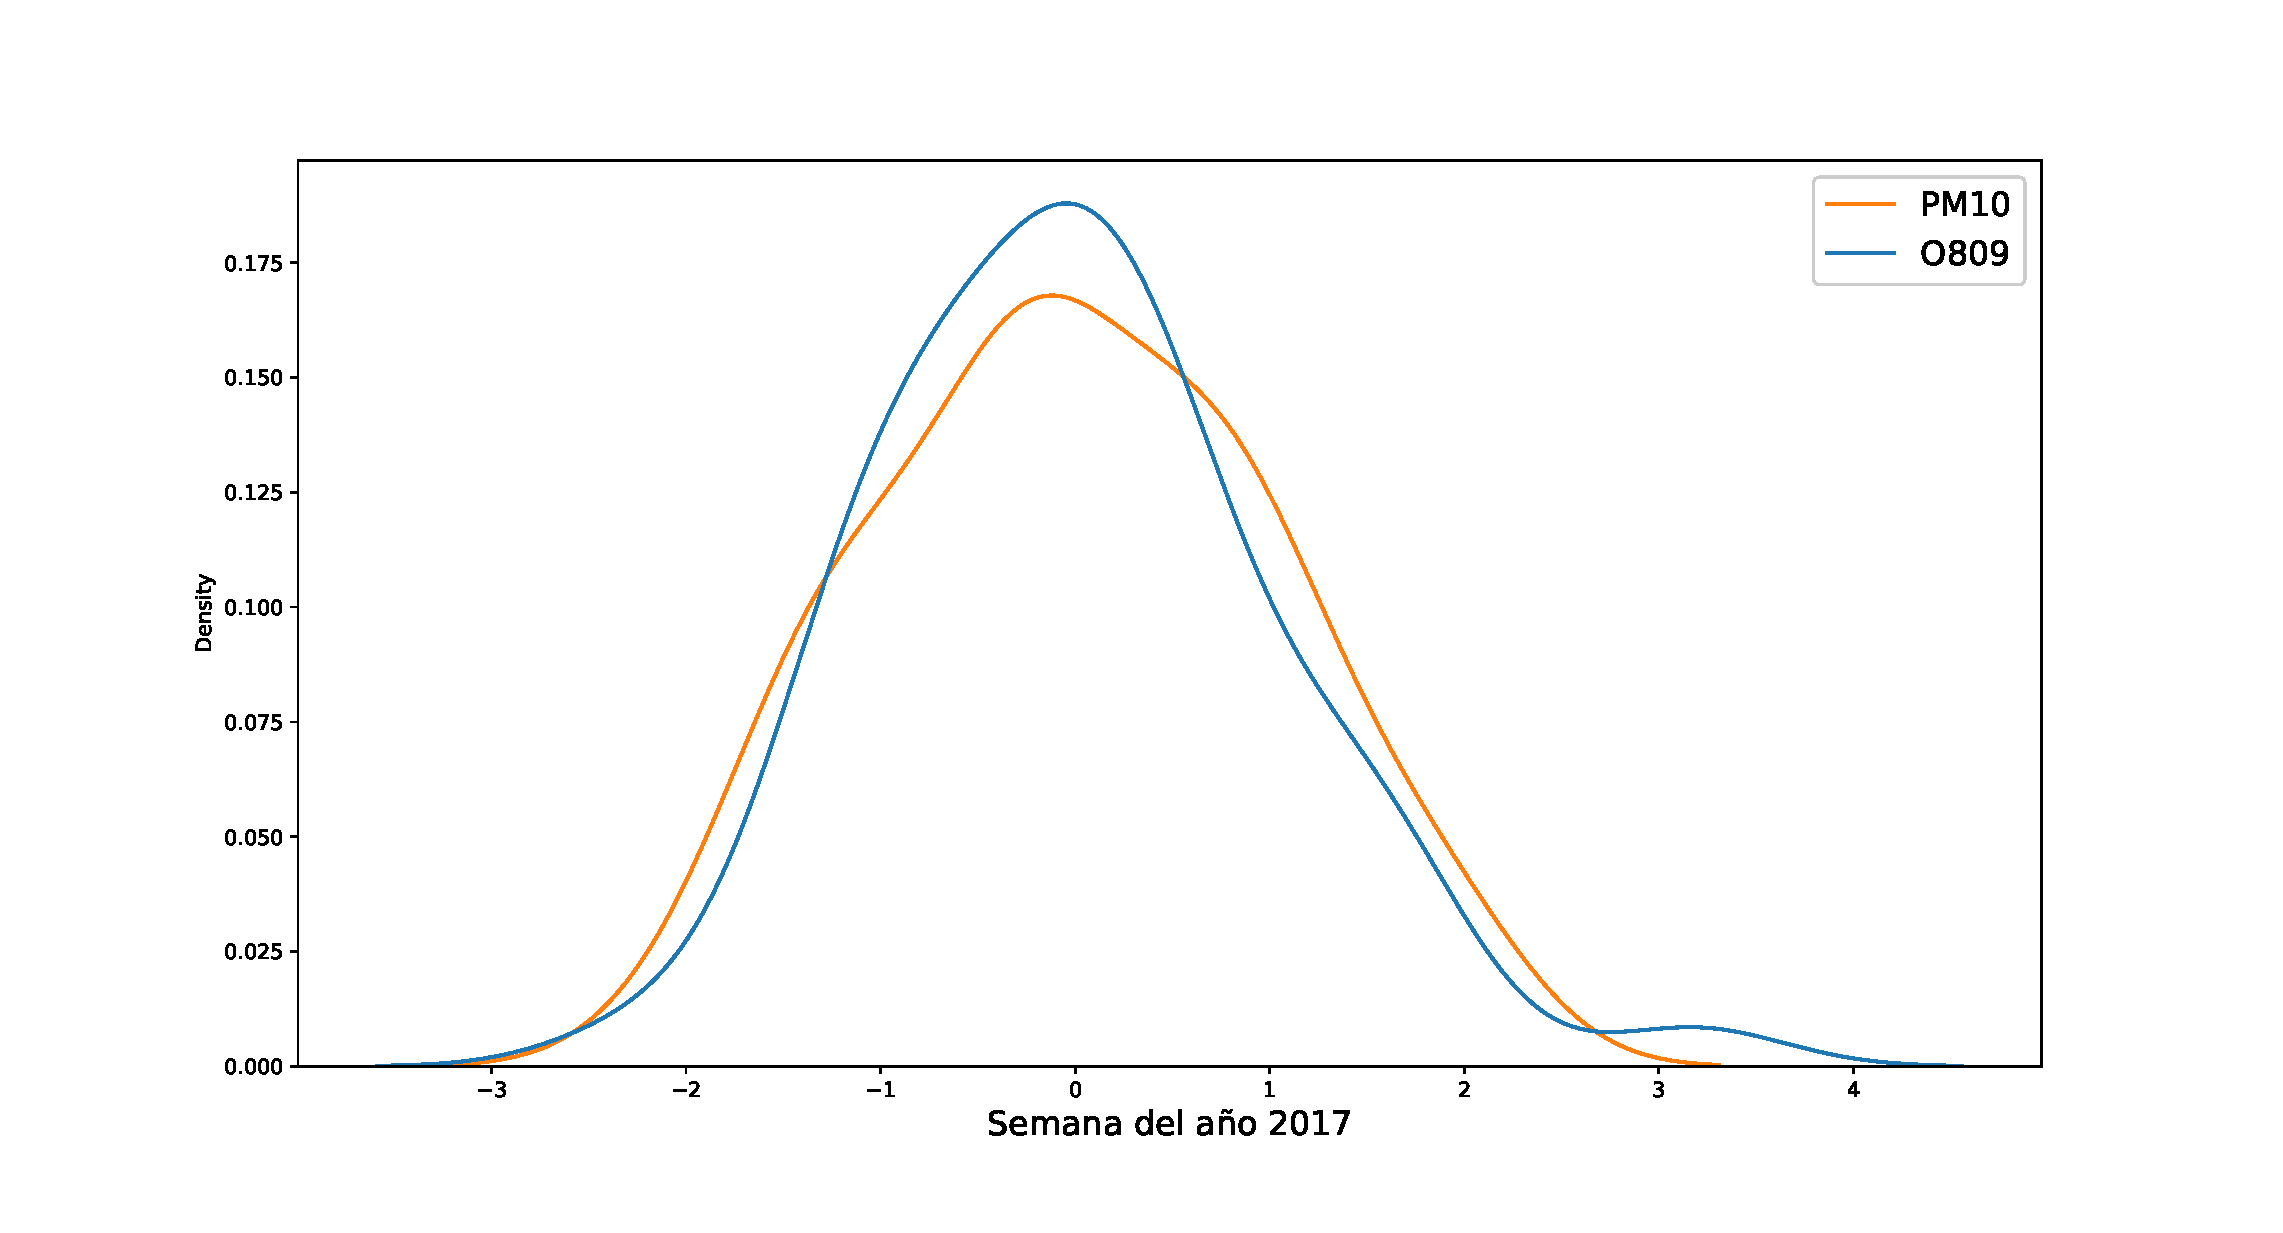
\includegraphics[trim=63 0 0 0,clip,width=0.55\textwidth]{PM10_O809_2017.eps}
   \end{center}
    \caption[Series de tiempo 2017 PM10 y O809]{Evolución de los niveles de PM10 y el número de egresos con la CIE O809 en el 2017.}
    \label{serie_de_tiempo_2017_PM10}
\end{figure}
\begin{figure}[h!]
\begin{center}
   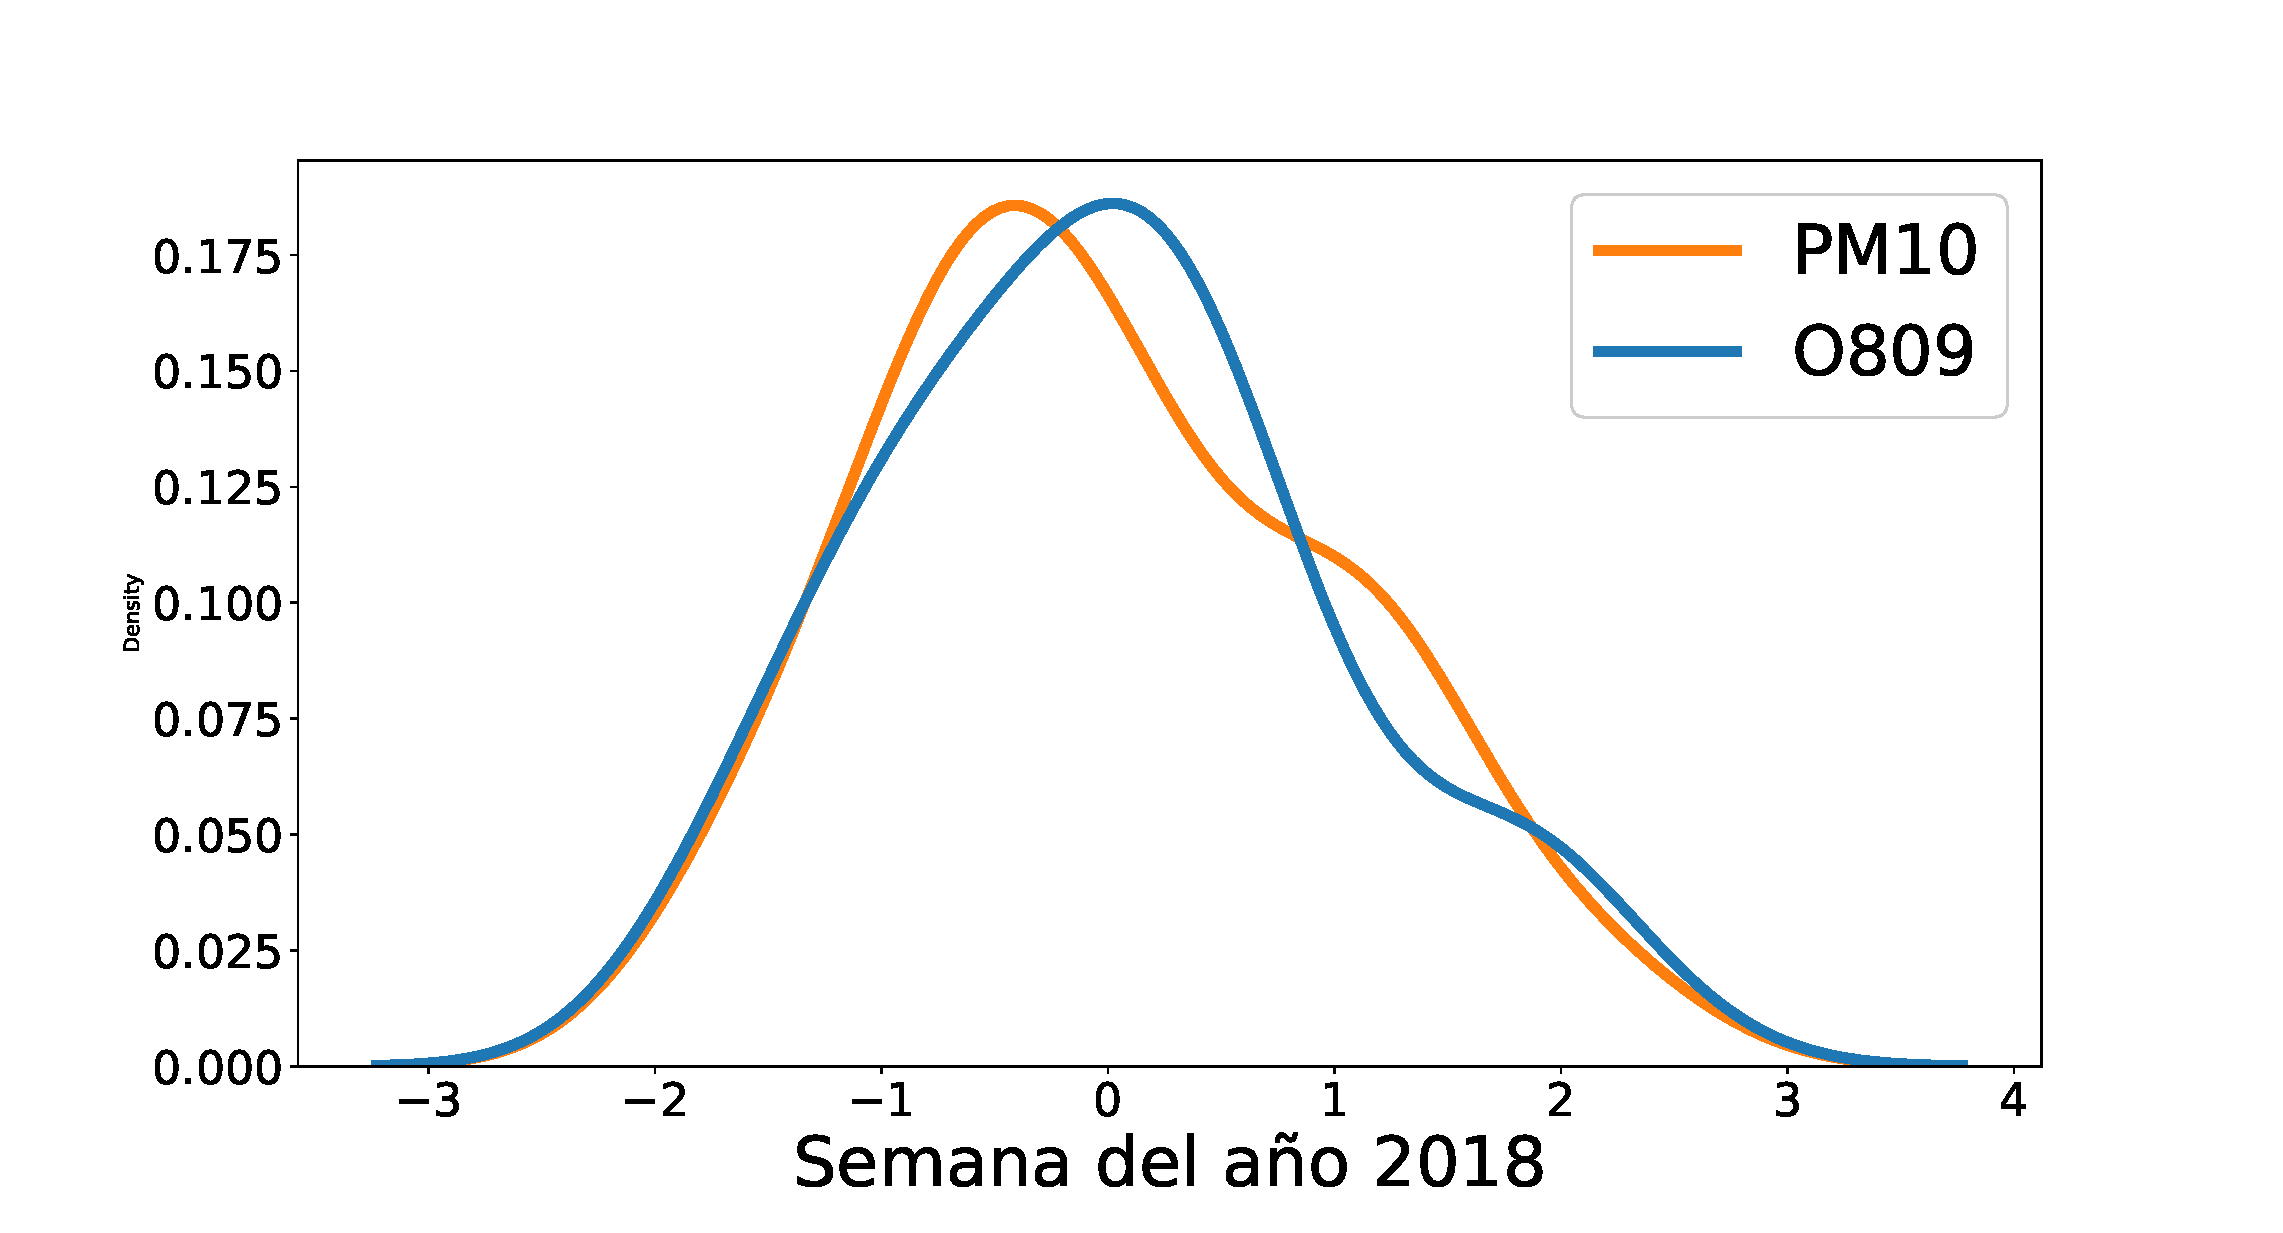
\includegraphics[trim=63 0 0 0,clip,width=0.55\textwidth]{PM10_O809_2018.eps}
   \end{center}
    \caption[Series de tiempo 2018 PM10 y O809]{Evolución de los niveles de PM10 y el número de egresos con la CIE O809 en el 2018.}
    \label{serie_de_tiempo_2018_PM10}
\end{figure}
\end{multicols}
\end{frame}
\begin{frame}{PM10 2017}
\begin{table}[hbt!]
\centering
\caption{Resultados obtenidos PM10 2017}
\label{tab:Resultados obtenidos PM10 2017}
\vspace{0.5cm}
\begin{tabular}{|c|c|c|c|c|}
	\hline
	CIE & $\rho$ & $R^2$ & Valor $p$ & $\epsilon$\\
	\hline
	O809 & -0.275 & 0.061 & 0.121 & 0.239 \\
	\hline
	O829 & 0.100 & 0.091 & 0.055 & 0.287 \\
	\hline
	O759 & -0.085 & 0.116 & 0.029 & 0.294 \\
	\hline
	O069 & -0.247 & 0.070 & 0.094 & 0.222 \\
	\hline
	K802 & 0.044 & 0.005 & 0.658 & 0.282 \\
	\hline
\end{tabular}
\footnotesize
\item{$\rho$ = Coeficiente de correlación de Pearson}
\item{$\epsilon$ = RMSE para medir el error}
\end{table}
\end{frame}
\begin{frame}{PM10 2017}
\begin{table}[hbt!]
\caption{Resultados regresión lineal múltiple PM10 2017}
\label{tab:RRLM PM10 2017}
\begin{center}
\begin{tabular}{lclc}
%\toprule
\textbf{Variable Dep.:}    &        $y$         & \textbf{  R$^2$:         } &     0.313   \\
\textbf{Modelo:}            &       OLS        & \textbf{Método:}           &  Mínimos cuadrados  \\
\textbf{Error:}            & 0.226  \\
%\bottomrule
\end{tabular}
\begin{tabular}{lcccccc}
               & \textbf{coef} & \textbf{std err} & \textbf{$t$} & \textbf{P$> |$t$|$} & \textbf{[0.025} & \textbf{0.975]}  \\
%\midrule
\textbf{const} &       0.5859  &        0.146     &     4.002  &         0.000        &        0.289    &        0.883     \\
\textbf{O809}  &      -0.3019  &        0.122     &    -2.472  &         0.018        &       -0.550    &       -0.054     \\
\textbf{O829}  &       0.2685  &        0.123     &     2.185  &         0.036        &        0.019    &        0.518     \\
\textbf{O759}  &      -0.2229  &        0.182     &    -1.222  &         0.230        &       -0.593    &        0.147     \\
\textbf{O069}  &      -0.1441  &        0.120     &    -1.200  &         0.238        &       -0.388    &        0.100     \\
\textbf{K802}  &      -0.0456  &        0.133     &    -0.344  &         0.733        &       -0.315    &        0.224     \\
%\bottomrule
\end{tabular}
\end{center}
\end{table}
\end{frame}
\begin{frame}{PM10 2018}
\begin{table}[hbt!]
\centering
\caption{Resultados obtenidos PM10 2018}
\label{tab:Resultados obtenidos PM10 2018}
\vspace{0.5cm}
\begin{tabular}{|c|c|c|c|c|}
	\hline
	CIE & $\rho$ & $R^2$ & Valor $p$ & $\epsilon$\\
	\hline
	O809 & -0.271 & 0.015 & 0.440 & 0.275 \\
	\hline
	O829 & 0.282 & 0.069 & 0.098 & 0.249 \\
	\hline
	K802 & 0.277 & 0.084 & 0.066 & 0.152 \\
	\hline
	O342 & -0.401 & 0.100 & 0.044 & 0.248 \\
	\hline
	N40X & -0.009 & 0.000 & 0.964 & 0.243 \\
	\hline
\end{tabular}
\footnotesize
\item{$\rho$ = Coeficiente de correlación de Pearson}
\item{$\epsilon$ = RMSE para medir el error}
\end{table}
\end{frame}
\begin{frame}{PM10 2018}
\begin{table}[hbt!]
\caption{Resultados regresión lineal múltiple PM10 2018}
\label{tab:RRLM PM10 2018}
\begin{center}
\begin{tabular}{lclc}
%\toprule
\textbf{Variable Dep.:}    &        $y$         & \textbf{  R$^2$:         } &     0.182   \\
\textbf{Modelo:}            &       OLS        & \textbf{Método:}           &  Mínimos cuadrados  \\
\textbf{Error:}            & 0.159  \\
%\bottomrule
\end{tabular}
\begin{tabular}{lcccccc}
               & \textbf{coef} & \textbf{std err} & \textbf{$t$} & \textbf{P$> |$t$|$} & \textbf{[0.025} & \textbf{0.975]}  \\
%\midrule
\textbf{const} &       0.3885  &        0.210     &     1.849  &         0.073        &       -0.038    &        0.815     \\
\textbf{O809}  &      -0.0114  &        0.188     &    -0.061  &         0.952        &       -0.392    &        0.370     \\
\textbf{O829}  &       0.0854  &        0.214     &     0.400  &         0.692        &       -0.349    &        0.520     \\
\textbf{K802}  &       0.3088  &        0.167     &     1.852  &         0.072        &       -0.030    &        0.647     \\
\textbf{O342}  &      -0.1708  &        0.208     &    -0.820  &         0.418        &       -0.593    &        0.252     \\
\textbf{N40X}  &      -0.1239  &        0.167     &    -0.740  &         0.464        &       -0.464    &        0.216     \\
%\bottomrule
\end{tabular}
\end{center}
\end{table}
\end{frame}

\subsection{Niveles de PM2.5}
\begin{frame}{Niveles de PM2.5}
\begin{multicols}{2}
\begin{figure}[h!]
\begin{center}
   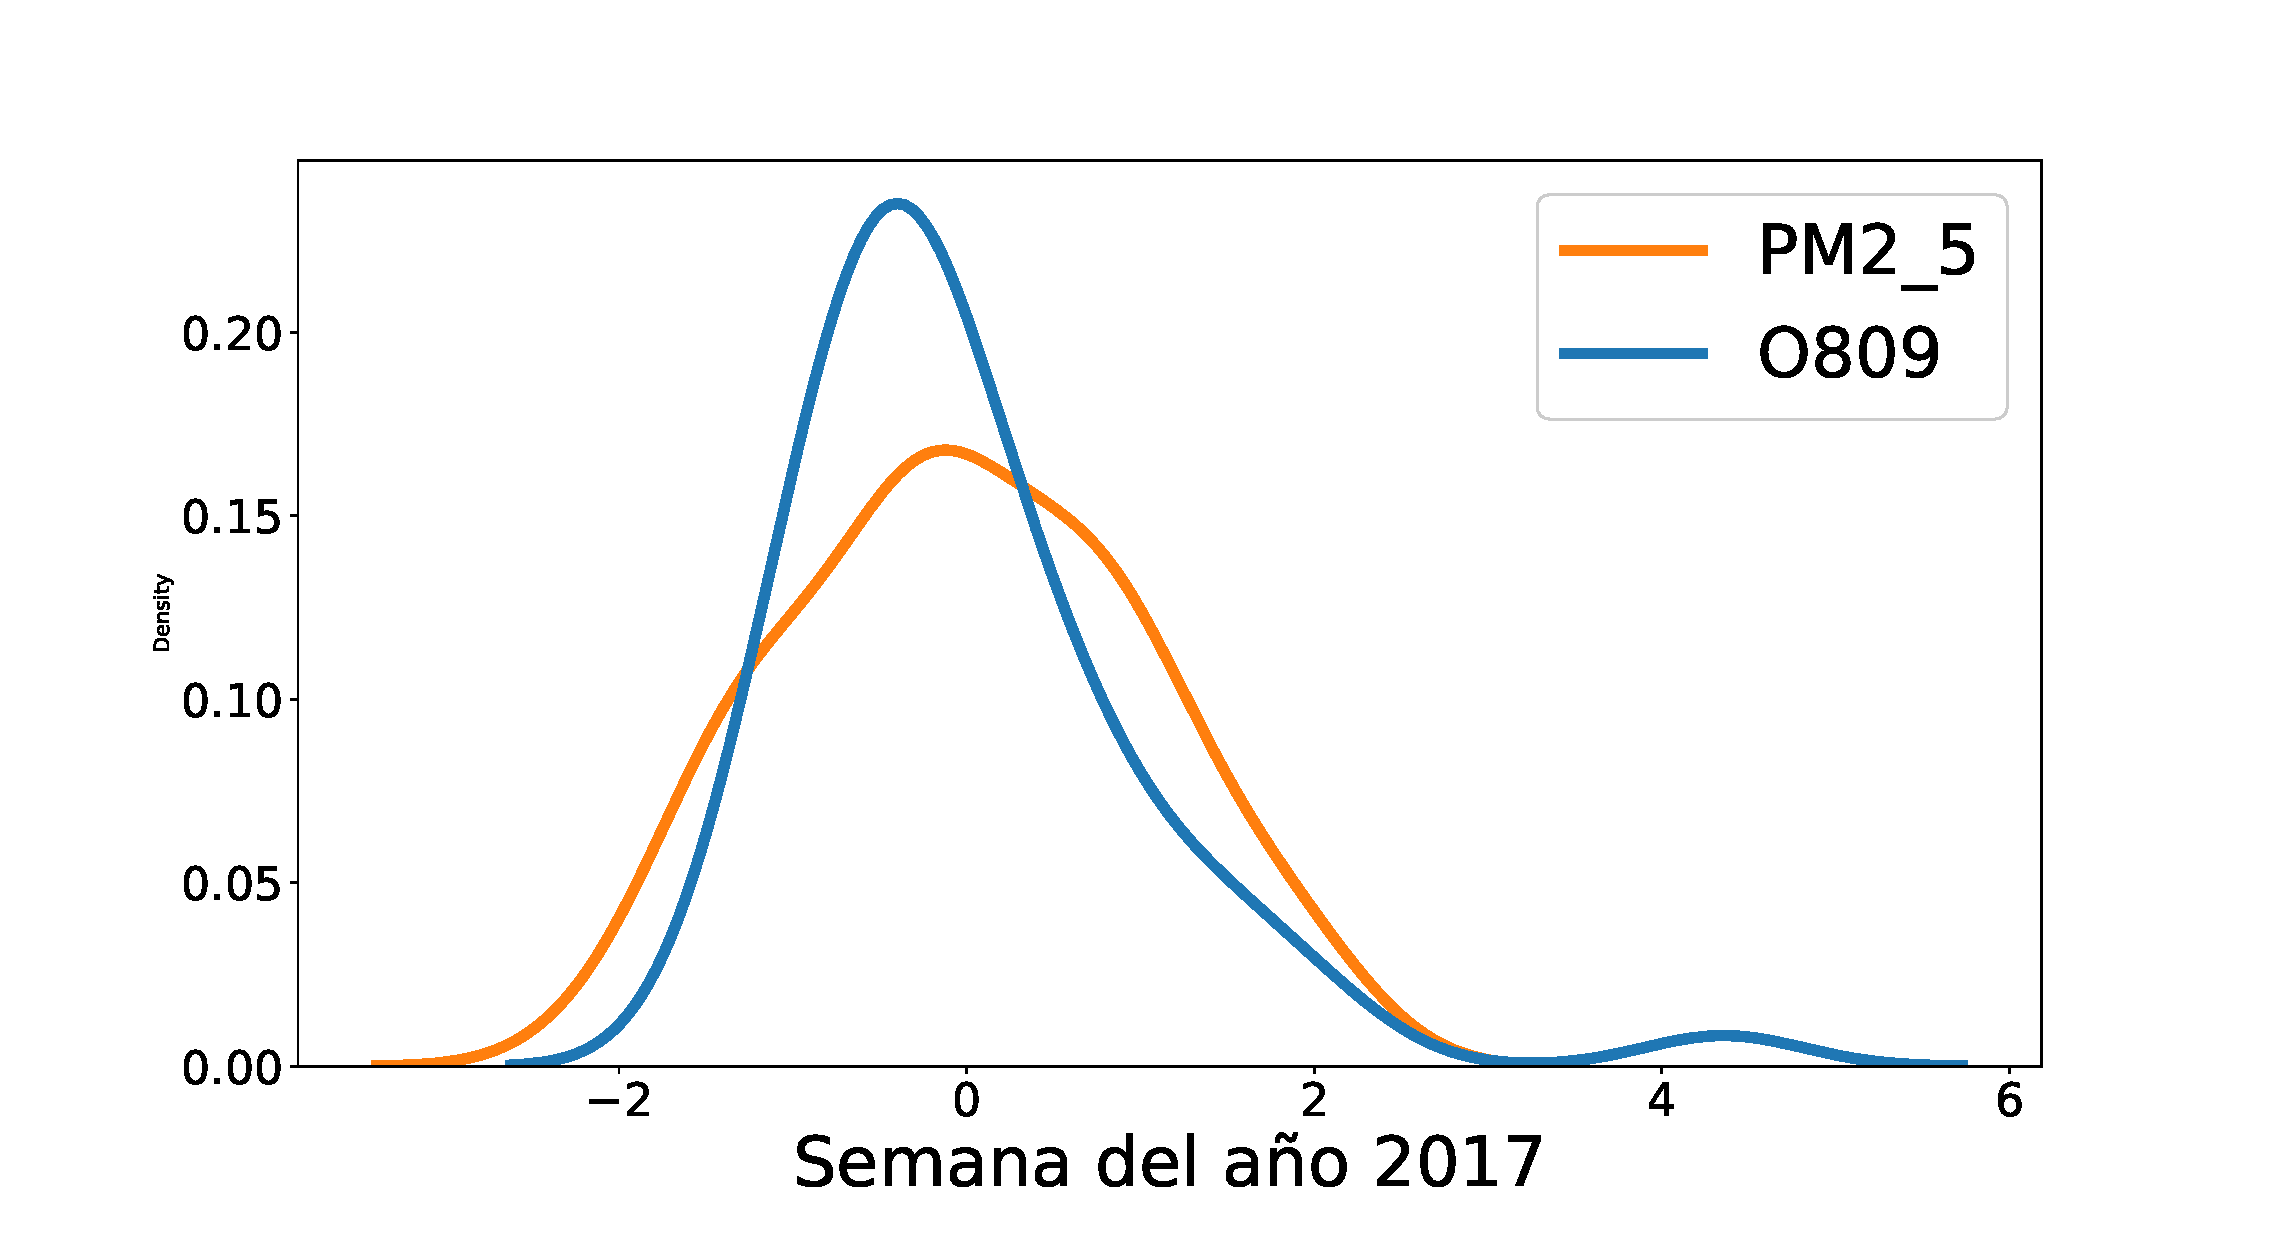
\includegraphics[trim=63 0 0 0,clip,width=0.55\textwidth]{PM2_5_O809_2017.eps}
   \end{center}
    \caption[Series de tiempo 2017 PM2.5 y O809]{Evolución de los niveles de PM2.5 y el número de egresos con la CIE O809 en el 2017.}
    \label{serie_de_tiempo_2017_PM25}
\end{figure}
\begin{figure}[h!]
\begin{center}
   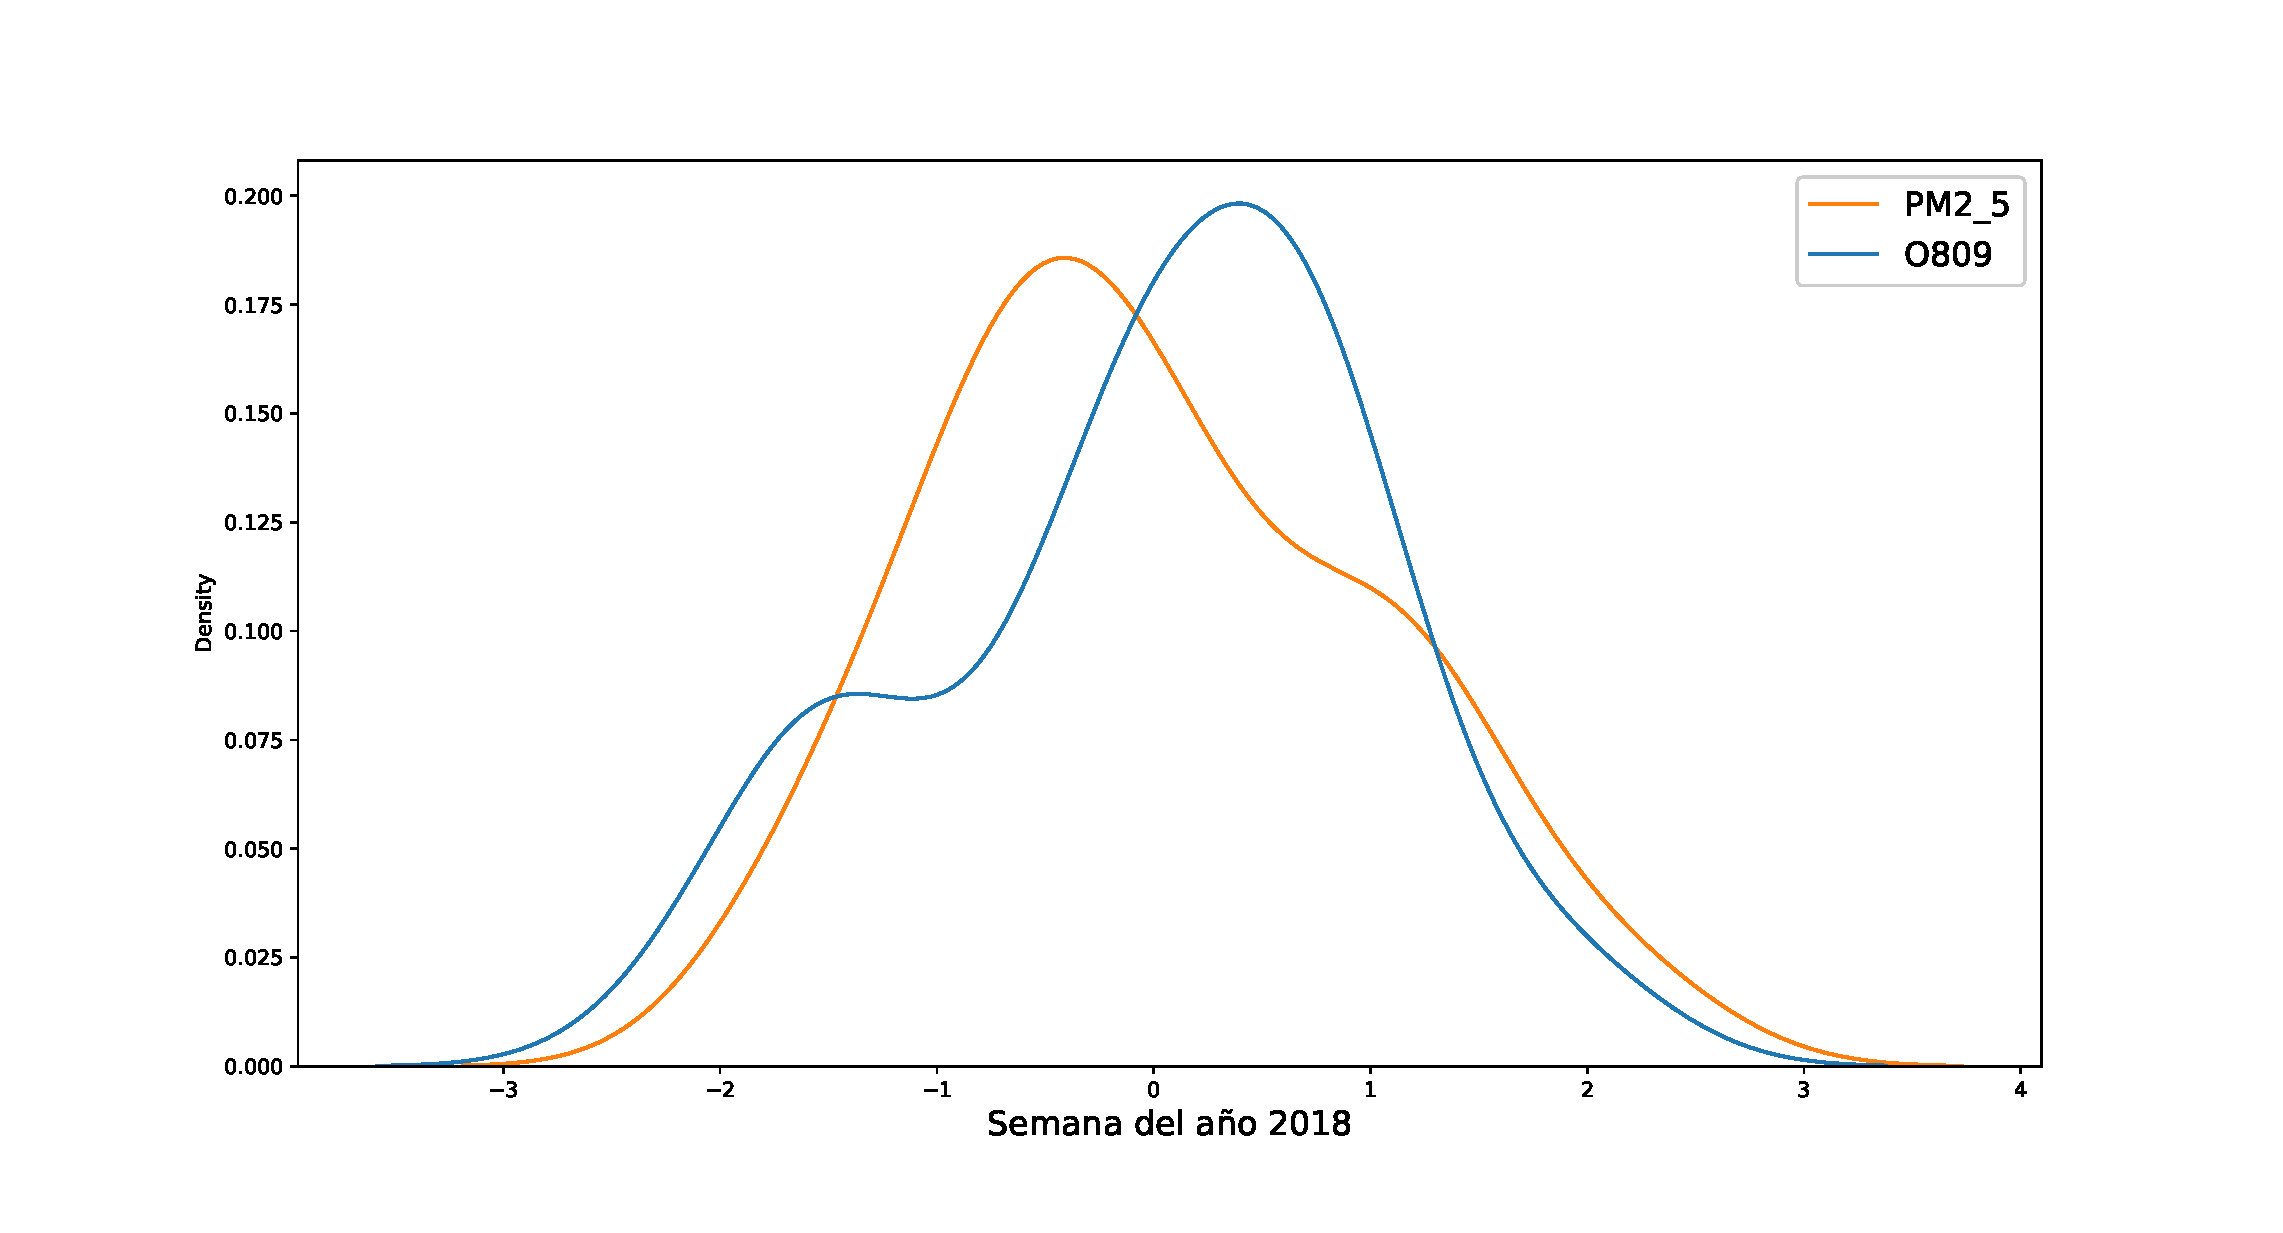
\includegraphics[trim=63 0 0 0,clip,width=0.55\textwidth]{PM2_5_O809_2018.eps}
   \end{center}
    \caption[Series de tiempo 2018 PM2.5 y O809]{Evolución de los niveles de PM2.5 y el número de egresos con la CIE O809 en el 2018.}
    \label{serie_de_tiempo_2018_PM25}
\end{figure}
\end{multicols}
\end{frame}
\begin{frame}{PM2.5 2017}
\begin{table}[hbt!]
\centering
\caption{Resultados obtenidos PM2.5 2017}
\label{tab:Resultados obtenidos PM2.5 2017}
\vspace{0.5cm}
\begin{tabular}{|c|c|c|c|c|}
	\hline
	CIE & $\rho$ & $R^2$ & Valor $p$ & $\epsilon$\\
	\hline
	O809 & -0.093 & 0.011 & 0.511 & 0.256 \\
	\hline
	O829 & 0.014 & 0.021 & 0.371 & 0.253 \\
	\hline
	O759 & -0.172 & 0.113 & 0.032 & 0.278 \\
	\hline
	O069 & -0.350 & 0.112 & 0.033 & 0.208 \\
	\hline
	K802 & 0.006 & 0.005 & 0.667 & 0.285 \\
	\hline
\end{tabular}
\footnotesize
\item{$\rho$ = Coeficiente de correlación de Pearson}
\item{$\epsilon$ = RMSE para medir el error}
\end{table}
\end{frame}
\begin{frame}{PM2.5 2017}
\begin{table}[hbt!]
\caption{Resultados regresión lineal múltiple PM2.5 2017}
\label{tab:RRLM PM2.5 2017}
\begin{center}
\begin{tabular}{lclc}
\textbf{Variable Dep.:}    &        $y$         & \textbf{  R$^2$:         } &     0.210   \\
\textbf{Modelo:}            &       OLS        & \textbf{Método:}           &  Mínimos cuadrados   \\
\textbf{Error:}            & 0.175  \\
\end{tabular}
\begin{tabular}{lcccccc}
               & \textbf{coef} & \textbf{std err} & \textbf{$t$} & \textbf{P$> |$t$|$} & \textbf{[0.025} & \textbf{0.975]}  \\
\textbf{const} &       0.5345  &        0.158     &     3.373  &         0.002        &        0.213    &        0.856     \\
\textbf{O809}  &      -0.1754  &        0.132     &    -1.327  &         0.193        &       -0.444    &        0.093     \\
\textbf{O829}  &       0.0701  &        0.133     &     0.527  &         0.602        &       -0.200    &        0.340     \\
\textbf{O759}  &      -0.2585  &        0.197     &    -1.309  &         0.199        &       -0.659    &        0.142     \\
\textbf{O069}  &      -0.2148  &        0.130     &    -1.652  &         0.108        &       -0.479    &        0.049     \\
\textbf{K802}  &      -0.1164  &        0.144     &    -0.811  &         0.423        &       -0.408    &        0.175     \\
\end{tabular}
\end{center}
\end{table}
\end{frame}
\begin{frame}{PM2.5 2018}
\begin{table}[hbt!]
\centering
\caption{Resultados obtenidos PM2.5 2018}
\label{tab:Resultados obtenidos PM2.5 2018}
\vspace{0.5cm}
\begin{tabular}{|c|c|c|c|c|}
	\hline
	CIE & $\rho$ & $R^2$ & Valor $p$ & $\epsilon$\\
	\hline
	O809 & -0.354 & 0.057 & 0.133 & 0.259 \\
	\hline
	O829 & 0.225 & 0.046 & 0.177 & 0.256 \\
	\hline
	K802 & 0.273 & 0.089 & 0.058 & 0.159 \\
	\hline
	O342 & -0.443 & 0.149 & 0.013 & 0.245 \\
	\hline
	N40X & -0.074 & 0.001 & 0.842 & 0.241 \\
	\hline
\end{tabular}
\footnotesize
\item{$\rho$ = Coeficiente de correlación de Pearson}
\item{$\epsilon$ = RMSE para medir el error}
\end{table}
\end{frame}
\begin{frame}{PM2.5 2018}
\begin{table}[hbt!]
\caption{Resultados regresión lineal múltiple PM2.5 2018}
\label{tab:RRLM PM2.5 2018}
\begin{center}
\begin{tabular}{lclc}
\textbf{Variable Dep.:}    &        $y$         & \textbf{  R$^2$:         } &     0.259   \\
\textbf{Modelo:}            &       OLS        & \textbf{Método:}           &  Mínimos cuadrados   \\
\textbf{Error:}            & 0.174  \\
\end{tabular}
\begin{tabular}{lcccccc}
               & \textbf{coef} & \textbf{std err} & \textbf{$t$} & \textbf{P$> |$t$|$} & \textbf{[0.025} & \textbf{0.975]}  \\
\textbf{const} &       0.7042  &        0.193     &     3.652  &         0.001        &        0.313    &        1.096     \\
\textbf{O809}  &      -0.0863  &        0.172     &    -0.501  &         0.620        &       -0.436    &        0.264     \\
\textbf{O829}  &      -0.1084  &        0.196     &    -0.553  &         0.584        &       -0.507    &        0.290     \\
\textbf{K802}  &       0.3006  &        0.153     &     1.964  &         0.058        &       -0.010    &        0.611     \\
\textbf{O342}  &      -0.3311  &        0.191     &    -1.733  &         0.092        &       -0.719    &        0.057     \\
\textbf{N40X}  &      -0.2053  &        0.154     &    -1.336  &         0.190        &       -0.517    &        0.107     \\
\end{tabular}
\end{center}
\end{table}
\end{frame}


\section{Conclusiones}

\begin{frame}{Conclusiones}
\begin{block}{Conclusión} \justifying
En las series de tiempo se observa que la cantidad de egresos de la mayoría de las CIE estudiadas presentan
una línea de evolución similar al contaminante PM10.
Además, se observó que para el estudio de las relaciones entre los contaminantes y las CIE se obtuvieron mejores resultados con los modelos de regresión lineal múltiple frente a los modelos de regresión lineal simple.
\end{block}
\end{frame}
\begin{frame}{Conclusiones}
\begin{block}{Trabajo a futuro} \justifying
\begin{itemize}
	\item Recolección de más datos de los niveles de contaminantes y de egresos para el estudio de años más recientes.
	\item Realizar un estudio de las relaciones de los niveles de determinados contaminantes y la cantidad de egresos por CIE empleando modelos de regresión lineal múltiple.
	\item Creación de un mapa interactivo donde se pueda observar por región los niveles de los contaminantes y la cantidad de egresos.
\end{itemize}
\end{block}
\end{frame}


\begin{frame}[allowframebreaks]{Referencias}
\bibliographystyle{mighelnat}
\tiny\bibliography{referencias}
\end{frame}


\appendix
\begin{frame}
		\transdissolve
		\begin{center}
			\Huge \textcolor{blue}{¡Gracias por su atención!}\\
			\bigskip
			\centering
			
\includegraphics[width=0.4\textwidth]{qr-code.png} \\
			\large Repositorio en línea
		\end{center}
\end{frame}


\end{document}